%%%%%%%%%%%%%%%%%%%%%%%%%%%%%%%%%%%%%%%%%%%%%%%%%%%%%%%%%%%%%%%%%%%%%%
% LaTeX Example: Project Report
%
% Source: http://www.howtotex.com
%
% Feel free to distribute this example, but please keep the referral
% to howtotex.com
% Date: March 2011 
% 
%%%%%%%%%%%%%%%%%%%%%%%%%%%%%%%%%%%%%%%%%%%%%%%%%%%%%%%%%%%%%%%%%%%%%%
% How to use writeLaTeX: 
%
% You edit the source code here on the left, and the preview on the
% right shows you the result within a few seconds.
%
% Bookmark this page and share the URL with your co-authors. They can
% edit at the same time!
%
% You can upload figures, bibliographies, custom classes and
% styles using the files menu.
%
% If you're new to LaTeX, the wikibook is a great place to start:
% http://en.wikibooks.org/wiki/LaTeX
%
%%%%%%%%%%%%%%%%%%%%%%%%%%%%%%%%%%%%%%%%%%%%%%%%%%%%%%%%%%%%%%%%%%%%%%
% Edit the title below to update the display in My Documents
%\title{Project Report}
%



%%% Preamble
\documentclass[paper=a4, fontsize=11pt]{scrartcl}
\usepackage{fourier}
\usepackage[table,xcdraw]{xcolor}
\usepackage[protrusion=true,expansion=true]{microtype}	
\usepackage{amsmath,amsfonts,amsthm} % Math packages
\usepackage{graphicx}	
\usepackage{url}
\usepackage{bookmark}

%%%Greek and english
\usepackage{polyglossia}
\setdefaultlanguage{greek}
\setotherlanguages{english}
%%% Bibliography 
\usepackage{biblatex}
\addbibresource{ref.bib}
 
%%%center tables
\usepackage{float}
\restylefloat{table}
%%%% algorithms
\usepackage{algorithm} 
\usepackage{algpseudocode} 

%%%%%images
\graphicspath{ {./images/} }


%%%fonts
\usepackage{fontspec}
\setmainfont{FreeSerif}
\setsansfont{FreeSans}
\setmonofont{FreeMono}



%%% Custom sectioning
\usepackage{sectsty}
\allsectionsfont{\centering \normalfont\scshape}


%%% Custom headers/footers (fancyhdr package)
\usepackage{fancyhdr}
\pagestyle{fancyplain}
\fancyhead{}											% No page header
\fancyfoot[L]{}											% Empty 
\fancyfoot[C]{}											% Empty
\fancyfoot[R]{\thepage}									% Pagenumbering
\renewcommand{\headrulewidth}{0pt}			% Remove header underlines
\renewcommand{\footrulewidth}{0pt}				% Remove footer underlines
\setlength{\headheight}{13.6pt}


%%% Equation and float numbering
\numberwithin{equation}{section}		% Equationnumbering: section.eq#
\numberwithin{figure}{section}			% Figurenumbering: section.fig#
\numberwithin{table}{section}				% Tablenumbering: section.tab#

%%%paragraph 
\setlength{\parindent}{1em}
\setlength{\parskip}{0.5em}

\usepackage{titlesec, lipsum}
\titleformat{\paragraph}[block]{\filcenter}{}{0pt}{}

%%% Maketitle metadata
\newcommand{\horrule}[1]{\rule{\linewidth}{#1}} 	% Horizontal rule



\title{
		%\vspace{-1in} 	
		\usefont{OT1}{bch}{b}{n}
		\normalfont \normalsize \textsc{Πανεπιστήμιο Ιωαννίνων Τμήμα Πληροφορικής και Τηλεπικοινωνίων} \\ [1em]
		\normalfont \normalsize \textsc{Αλγόριθμοι και πολυπλοκότητα} \\ [1em]
		\horrule{0.5pt} \\[0.4cm]
		\huge To πρόβλημα της μέγιστης υποακολουθίας, θεωρητική και εμπειρική μελέτη. \\
		\horrule{2pt} \\[0.5cm]
}
\author{
		\normalfont 								\normalsize
        Όνομα φοιτητή\\[-1pt]		\normalsize
        \today
}
\date{}

%%% Begin document
\begin{document}

\maketitle
%%% Abstract

\section*{Περίληψη}
	Η πολυπλοκότητα ενός αλγορίθμου προσδιορίζει τον χρόνο που θα χρειαστεί για μία συγκεκριμένη διεργασία. Σε αυτήν την τεχνική αναφορά εξετάζεται το πρόβλημα της μέγιστης υποακολουθίας και γίνεται σύγκριση μεταξύ τριών διαφορετικών αλγορίθμων για την επίλυση του.
	
\section{Εισαγωγή}
    Το πρόβλημα της μέγιστης υποακολουθίας (maximum subarray) είναι ένα πρόβλημα στο
    οποίο δίνεται μια ακολουθία τιμών (αρνητικές, θετικές ή μηδέν) και ζητείται να βρεθεί η συνεχόμενη σειρά τιμών της ακολουθίας που δίνει το μεγαλύτερο δυνατό άθροισμα. 
    
    Ο απλοϊκός τρόπος επίλυσης είναι πρακτικά ένας αλγόριθμος ωμής δύναμης με πολυπλοκότητα $\mathcal{O}(n^{3})$. Ο βελτιωμένος αλγόριθμος δεν υπολογίζει ξανά όλα τα αθροίσματα αφού τα έχει υπολογίσει εκ' των προτέρων και η πολυπολοκότητα του είναι $\mathcal{O}(n^{2})$. Τέλος ο αλγόριθμος του kadane είναι ο αποδοτικότερος τρόπος για την επίλυση με πολυπλοκότητα $\mathcal{O}(n)$.
    
\section{Αποτελέσματα}
Για την συγγραφή των πειραμάτων χρησιμοποιήθηκε η python 3.9.7 και το Visual Studio Code. Τα χαρακτηριστικά του υπολογιστή είναι i7 3632QM (2.2 GHz), 8 GB DDR3 (1600 MHz). Για την οπτικοποίηση των αποτελεσμάτων χρησιμοποιήθηκε η βιβλιοθήκη matplotlib. Στον πίνακα~\ref{tab:benchmarks} υπάρχουν οι χρόνοι για κάθε αλγόριθμο. Στην γραφική παράσταση~\ref{fig:results_log} φαίνεται η σύγκριση των αλγορίθμων σε λογαριθμική κλίμακα.

\begin{table}[htbp]
  \centering
  \caption{Πίνακας χρονομετρήσεων}
    \begin{tabular}{lrrrrr}
          & \multicolumn{5}{c}{\textbf{Χρόνος (s)}} \\
    \textbf{Αλγόριθμος} & \textbf{n =  10} & \textbf{n =  100} & \textbf{n =  200} & \textbf{n =  500} & \textbf{n =  1000} \\
    \textbf{Ωμής δύναμης} & 7.10E-05 & 0.028544 & 0.199864 & 3.322954 & 28.34849 \\
    \textbf{Βελτιωμένος} & 3.48E-05 & 0.001919 & 0.007412 & 0.047613 & 0.184395 \\
    \textbf{Kadane} & 2.45E-05 & 7.51E-05 & 0.000134 & 0.000316 & 0.000691 \\
    \end{tabular}%
  \label{tab:benchmarks}%
\end{table}%



\begin{figure}[h]
    \caption{Αποτελέσματα σε λογαριθμική κλίμακα.}
    \centering
    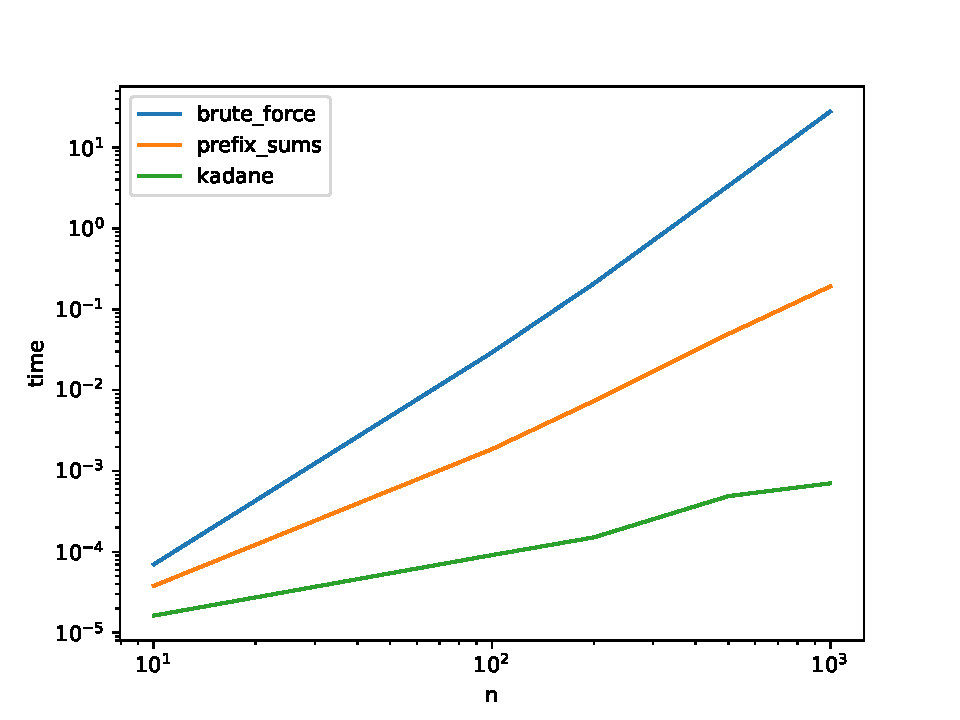
\includegraphics[width=0.7\textwidth]{algorithms_comparisson.pdf}
    \label{fig:results_log}
\end{figure}

\section{Συμπεράσματα}
Η σύγκριση του χρόνου των αλγορίθμων μας δείχνει ξεκάθαρα τις επιπτώσεις που έχει η χρήση ενός μη αποδοτικού αλγορίθμου για κάποιο πρόβλημα στο οποίο υπάρχουν πιο αποδοτικές λύσεις.

% \printbibliography
\end{document}